\documentclass[11pt,a4paper]{article}

\usepackage[slovene]{babel}
\usepackage{color}
\usepackage{graphicx}
\usepackage{verbatim}
\usepackage{amsmath}
\usepackage{tikz}
\usepackage{esvect}
\usepackage{float}
\usepackage{xcolor}
\usepackage{listings}
\usepackage{xparse}
\usepackage[backend=bibtex]{biblatex}
\usepackage{subfloat}
\usepackage{subfig}

% code styling
\lstset{language=Python,keywordstyle={\bfseries \color{blue}}}
\NewDocumentCommand{\codeword}{v}{%
	\texttt{\textcolor{blue}{#1}}%
}

\addbibresource{viri.bib}

\begin{document}

\title{Povratek kapsule v ozra\v cje}
\author{\v Ziga Pata\v cko Koderman}
\date{\today}

\clearpage\maketitle
\thispagestyle{empty}
\pagebreak

\tableofcontents
\pagebreak

\section{Uvod}

Pri povratku kapsule iz vesolja mora ta drasti\v cno upo\v casniti. Veliko ve\v cino svoje kineti\v cne energije se znebi z pomo\v cjo Zemljine atmosfere in jo s svojim toplotnim \v s\v citom pretvori v toploto. Ko se kapsula primerno upo\v casni odpre padala za ne\v znej\v si pristanek.

V tem poro\v cilu posku\v samo dolo\v citi optimalen kot za vstop v atmosfero. Pri prestrmem vstopu v atmosfero kapsula zgori, astronavte pa ubije \v ze prevelik pospe\v sek. Premajhen kot vstopa pa lahko vodi v odboj kapsule od Zemljine atmosfere.

Natan\v cneje se poro\v cilo posve\v ca kotu, pod katerim so v Zemljino atmosfero morale vstopati kapsule Apollo pri povratku z Lune.

\pagebreak

\section{Fizikalno ozadje}
\subsection{Sile}

Za opis gibanja kapsule pri ponovnem vstopu v atmosfero bomo upo\v stevali silo gravitacije planeta na kapsulo $F_g$, silo zra\v cnega upora $F_u$ ter silo vzgona $F_v$. Za te velja:


\begin{equation}
F_g(h) = m g(h)
\end{equation}

\begin{equation}
F_u(v, h) = k_{u}\rho (h) v^2
\end{equation}

\begin{equation}
F_v(h) = V \rho(h)
\end{equation} \\
Kjer sta gravitacijski pospe\v sek $g(h)$ ter koeficient upora $k_u$:

\begin{equation}
g(h) = g_0 (\frac{r}{r+h})^2
\end{equation}

\begin{equation}
k_u = \frac{Sc_u}{2}
\end{equation}
kjer $c_u$ predstavlja koeficient upora oblike kapsule. \\ \\

Gostoto zraka v odvisnosti od vi\v sine pa izpeljemo:
$$ \frac{dp}{dh} = -\rho g $$
$$ \rho = \frac{n M }{V} $$
Z uporabo plinskega zakona za idealni plin $ pV = nRT $ zamenjamo $n$:
$$ \rho = \frac{pM}{RT} $$
In vstavimo v prvo ena\v cbo:
$$ \frac{1}{p} dp = - \frac{Mg}{RT} dh$$
Po integraciji ostane:
$$ p = p_0 e ^{-\frac{h}{H}} $$
kjer je $H = \frac{RT}{Mg}$ vi\v sina, pri kateri se tlak zmanj\v sa za $\frac{1}{e}$. Ker pa sta tlak in gostota zraka premo sorazmerna, lahko uporabimo isti $H$ tudi za gostoto. Sledi:
\begin{equation}
\rho(h) = \rho_0 e^{-\frac{h}{H}}
\end{equation}

\subsection{Ena\v cbe gibanja in koordinatni sistem}

Za la\v zje obravnavanje ena\v cb in numeri\v cno integriranje bomo uporabili koordinatni sistem, ki ima izhodi\v sce v sredi\v s\v cu plovila, njegova $x$ os pa je pravokotna na zveznico med sredi\v s\v cem planeta ter kapsulo.

\vspace{0.5cm}

\begin{figure}[H]
	\centering
	\begin{tikzpicture}[scale=.95]
	\draw (0, 0) circle (4);
	\draw[dashed] (0, 0) circle (4.2);
	\draw[->, rotate=-30] (0,0) -- (0, 4) node[below] {$r$}; % r
	\draw[->, rotate=-30] (0,4) -- node[above] {$h$}  (0, 5); % h
	\draw[->, rotate=-30] (0,5) -- (2, 5) node[below] {$x$}; % x
	\draw[->, rotate=-30] (0,5) -- (0, 7) node[above] {$y$}; % y
	\draw[->, rotate=-30] (0,5) -- (1.8, 6.25) node[above]{$\vv{v}$}; % v
	\draw [->, rotate=-30](0,5) -- (1.2,5) arc (0:35:1.2cm) node[below left]{$-\gamma$};
	\draw[dashed] (0,0) -- (0, 7); % x fixed
	\draw [dashed, ->, rotate=90] (0,0) -- (2,0) node[below right]{$\phi$} arc (0:-30:2cm);
	\end{tikzpicture}
	\caption{Relativni koordinatni sistem kapsule glede na planet}
	\label{fig:sp2d}
\end{figure}

Glede na novi kordinatni sistem zapi\v semo diferencialne ena\v cbe gibanja. Hitrost v horizontalni smeri je
\begin{equation}
	\dot{x} = v * cos(\gamma),
\end{equation}
v vertikalni pa
\begin{equation}
	\dot{h} = v * sin(\gamma).
\end{equation}
Absolutni pospe\v sek sestavljata vertikalna komponenta $g$ ter sila upora:
\begin{equation}
	\dot{v} = g*sin(\gamma) - \rho(h) v^2 k_u.
\end{equation}
Odvod kota $\gamma$ pa izpeljemo. V pozitivno smer nanj vpljiva gravitacijski pospe\v sek z velikostjo $g\frac{cos(\gamma)}{v}$. V negativno smer na kot $\gamma$ vpljiva premik zaradi vztrajnostnega momenta. Velikost tega \v clena je odvisna od krivinskega radija planeta in se glasi $ -v \frac{cos(\gamma)}{r}$.\\ \\
Za upo\v stevanje sile vzgona pa potrebujemo razmerje med vzgonom in uporom (ang. \textit{lift-to-drag ratio}). \\\\
Sprememba kota $\gamma$ se torej glasi
\begin{equation}
	\dot{\gamma} = g\frac{cos(\gamma)}{v}  - v \frac{cos(\gamma)}{r} - \alpha v k*\rho(h)
\end{equation}
kjer je $\alpha$ razmerje med silo vzgona in silo upora kapsule.\\

Te \v stiri ena\v cbe zadostujejo za simulacijo leta kapsule. Za la\v zje risanje sheme  leta kapsule skozi atmosfero pa bomo spremljali \v se vrednost kota $\phi$ v odvisnosti od \v casa.
\begin{equation}
	\dot{\phi} = v \frac{cos(b)}{r+h}
\end{equation}
\newpage

\section{Simulacija}
Spremenljivke v simulaciji so torej $\{x, h, v, \beta, \phi \}$, potek gibanja kapsule pa je odvisen od njihovih za\v cetnih vrednosti $x_0 = 0$, $h_0$, $v_0$ ter $\beta_0 = 0$. Nas pa posebaj zanima za\v cetni kot $\phi_0$, ki nam pove, s kak\v snim za\v cetnim kotom se zaletimo v atmosfero.

Od tega je odvisno s kak\v snim pospe\v skom nas bo atmosfera zaustavljala in ali se bomo morebiti odbili nazaj v vesolje. Kriteriji za uspe\v sen povratek bodo:
\begin{itemize}
	\item najve\v cji pospe\v sek bo manj\v si od $10 g$,
	\item na tleh bo kapsula pristala v manj kot $30$ min ($1800$ s).
\end{itemize}
Posebej pa nas zanimajo koti, pri katerih sta maksimalna mo\v c in pospe\v sek najmanjsa. \\

Za simulacijo gibanja kapsule bomo uporabili funkcijo \codeword{odeint()} iz Pythonove knji\v znjice scypy. Tej podamo funkcijo, ki ra\v cuna odvode \v zeljenih spremenljivk v danih to\v ckah. V na\v sem primeru poenostavljena razli\v cica te funkcije izgleda takole: \\
\begin{lstlisting}
def movement(parametres, t, sim):
	x, h, v, b, phi = parametres

	dxdt = v * np.cos(b)
	dhdt = -v * np.sin(b)
	dvdt = sim.g(h) * np.sin(b) - sim.rho(h) *
			sim.capsule['k'] * v ** 2
			
	dbdt = sim.g(h) * np.cos(b) / v - v *
			np.cos(b) / sim.planet['r']
			
	if not sim.ignore_buoyancy:
		dbdt -= sim.rho(h) * v *
			sim.capsule['k'] *
			sim.capsule['l2d']
			
	dphidt = v * np.cos(b) /
			(sim.planet['r'] + h)

	return [dxdt, dhdt, dvdt, dbdt, dphidt]
\end{lstlisting}
\clearpage
%\vspace{0.5cm}

Da najdemo optimalen vstopni kot, bomo predpostavili, da vstopa kapsule ne moremo kontrolirati natan\v cneje kot na $0.01^\circ $. Tako se lahko s korakom $0.01^\circ $ sprehodimo med kotoma $0^\circ$ in $15^\circ$ (ki je zagotovo prevelik za povratek kapsule iz vesolja). \\

\section{Primer povratka Apollo kapsule}
Da preverimo pravilnost na\v se simulacije, bomo za za\v cetno hitrost in druge podatke o kapsuli vzeli kar pribli\v zne vrednosti za kapsule poletov Apollo:

\begin{table}[H]
	\centering
	\caption{Lastnosti Apollo kapsule \cite{lift-and-drag-of-apollo-command-module} \cite{command-module-overview} \cite{entry-aerodynamics} }
	\vspace{0.3cm}
	\def\arraystretch{1.5}
	\begin{tabular}{l|r}
		$h_0$ & $100 \; km$ \\
		$v_0$ & $11000 \; \frac{m}{s}$ \\
		$k_{upora}$ & $1.2$ \\
		$S$ & $12 \; m^2$ \\
		$m$ & $5357 \; kg $\\
		$\alpha$ & $0.225$ \\
		$v_{padalo}$ & $111 \; \frac{m}{s}$
	\end{tabular}
	\def\arraystretch{1}
\end{table}
\vspace{0.4cm}
Potrebijemo tudi podatke o Zemlji in njeni atmosferi:
\begin{table}[H]
	\centering
	\caption{Lastnosti Zemlje \cite{earths-atmosphere}}
	\vspace{0.3cm}
	\def\arraystretch{1.5}
	\begin{tabular}{l|r}
		$g_0$ & $9.81 \; \frac{m}{s^2}$ \\
		$r$ & $3396.2 \; km$ \\
		$T$ & $236.7 K$ \\
		$M$ & $28.95$ \\
		$\rho_0$ & $1.225 \frac{kg}{m^3} $
	\end{tabular}
	\def\arraystretch{1}
\end{table}

\clearpage

\subsection{Rezultati}
Simulacijo za razli\v cne kote po\v zenemo z in brez upo\v stevanja sile vzgona. Med skrajnima kotoma, ki \v se vodita v uspe\v sen povratek na Zemljo, izpi\v semo \v se nekaj vmesnih vstopnih kotov ter pripadajo\v cih skrajnih vrednosti:


\begin{table}[H]
	\centering
	\caption{Skrajne vrednosti pri povratku pri razli\v cnih za\v cetnih kotih brez upo\v stevanja sile vzgona}
	\vspace{0.3cm}
	\def\arraystretch{1.5}
	\begin{tabular}{l|lll}
	$ \phi_0\ [^\circ] $ & $a_{max}\ [g]$ & $ P_{max} \ [kW] $ \\
	\hline
	$ 4.55 $ & $ 8.60 $ & $ 354.73 $ \\
	$ 4.75 $ & $ 6.53 $ & $ 475.41 $ \\
	$ 4.95 $ & $ 7.74 $ & $ 645.25 $ \\
	$ 5.12 $ & $ 9.96 $ & $ 789.47 $
	\end{tabular}
	\def\arraystretch{1}
\end{table}


\begin{table}[H]
	\centering
	\caption{Skrajne vrednosti pri povratku pri razli\v cnih za\v cetnih kotih z upo\v stevanja sile vzgona}
	\vspace{0.3cm}
	\def\arraystretch{1.5}
	\begin{tabular}{l|lll}
	$ \phi_0\ [^\circ] $ & $a_{max}\ [g]$ & $ P_{max} \ [kW] $ \\
	\hline
	$ 5.51 $ & $ 6.55 $ & $ 622.10 $ \\
	$ 5.71 $ & $ 7.69 $ & $ 721.20 $ \\
	$ 5.91 $ & $ 8.88 $ & $ 820.69 $ \\
	$ 6.09 $ & $ 9.97 $ & $ 911.50 $
	\end{tabular}
	\def\arraystretch{1}
\end{table}

Opazimo, da se pri upo\v stevanju sile vzgona vstopni kot spremeni za priblji\v zno $ 1^\circ $, sama \v sirina intervala pa se ne spremeni bistveno.


Idealni kot za povratek v atmosfero z upo\v stevanjem sile vzgona je torej priblji\v zno $ 5.8^\circ $. Tako se v atmosfero ne zaletimo prestrmo, hkrati pa ne tvegamo preve\v c, da bi ze zarad napake odbili od atmosfere. Graf vi\v sine v odvisnosti od prepotovane razdalje pri tem za\v cetnem kotu ka\v ze, da se kapsula rahlo odbije, pa potem hitro spet vrne v re\v zim padanja.

\begin{figure}[H]
  \begin{center}
  	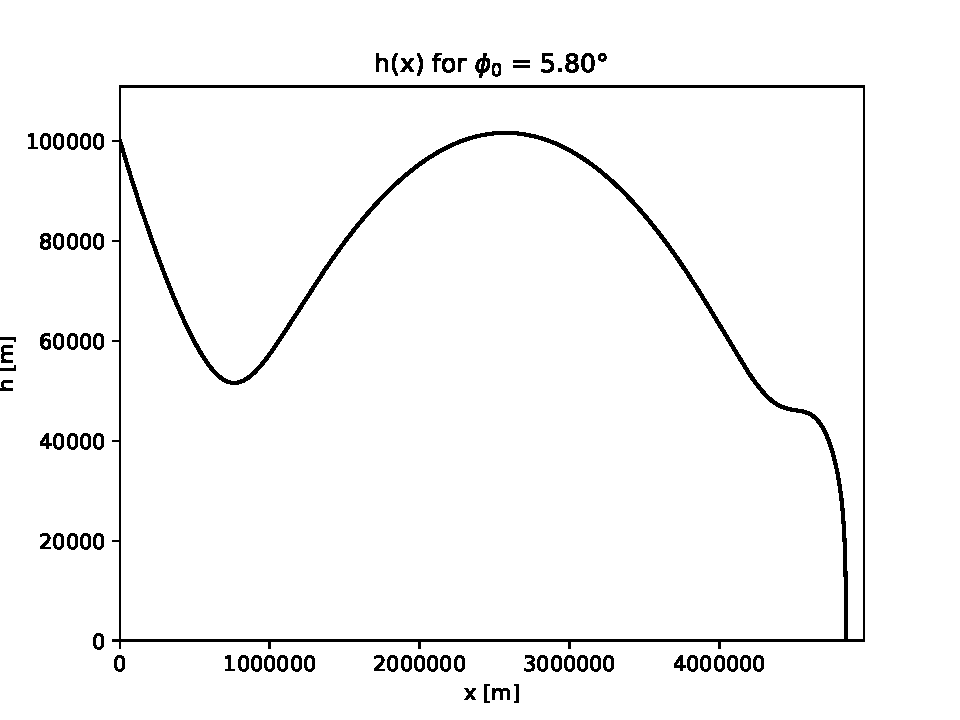
\includegraphics[width=12cm]{5_8_height_over_x.pdf}
    \caption{Graf vi\v sine v odvisnosti od prepotovane razdalje za vstopni kot $ 5.8^\circ $}
  \end{center}
\end{figure}

Tako odboj kot sam vstopni kot se ne razlikujeta pretirano od resni\v cnih podatkov za povratek kapsule Apollo 4 \cite{entry-aerodynamics}. Ta se je vrnila z vstopnim kotom $ 6.9^\circ $ in prav tako pristala \v sele po kraj\v sem odboju.


\begin{figure}[H]
	\begin{center}
		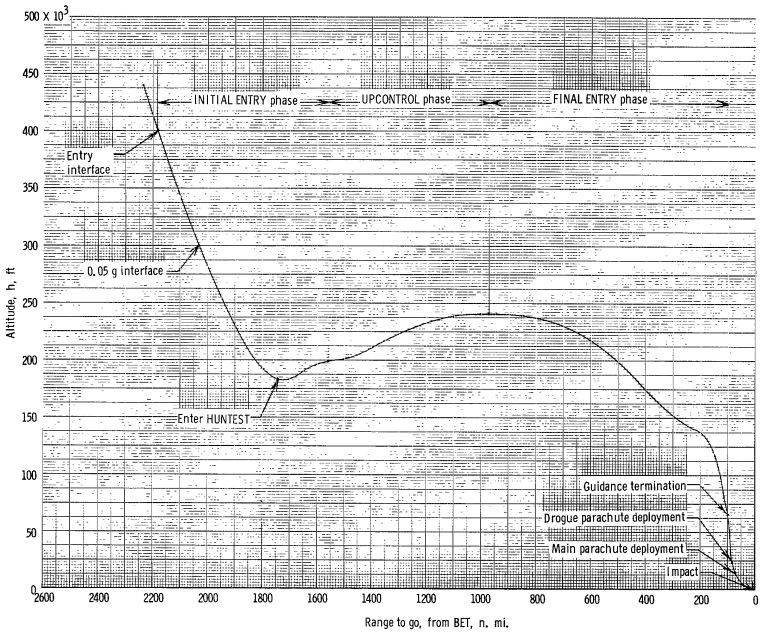
\includegraphics[width=12cm]{apollo4_return_trajectory.png}
		\caption{Graf vi\v sine v odvisnosti od prepotovane razdalje pri povratku kapsule Apollo 4}
	\end{center}
\end{figure}

Primerljivi sta tudi razdalji, ki jih kapsuli prepotujeta pred pristankom. Apollo 4 prepotuje priblji\v zno $ 4800\ km $ ($ 2600 $ navti\v cnih milj), kapsula iz na\v se simulacije pa priblji\v zno $ 4900\ km $.

\begin{figure}[H]
	\begin{center}
		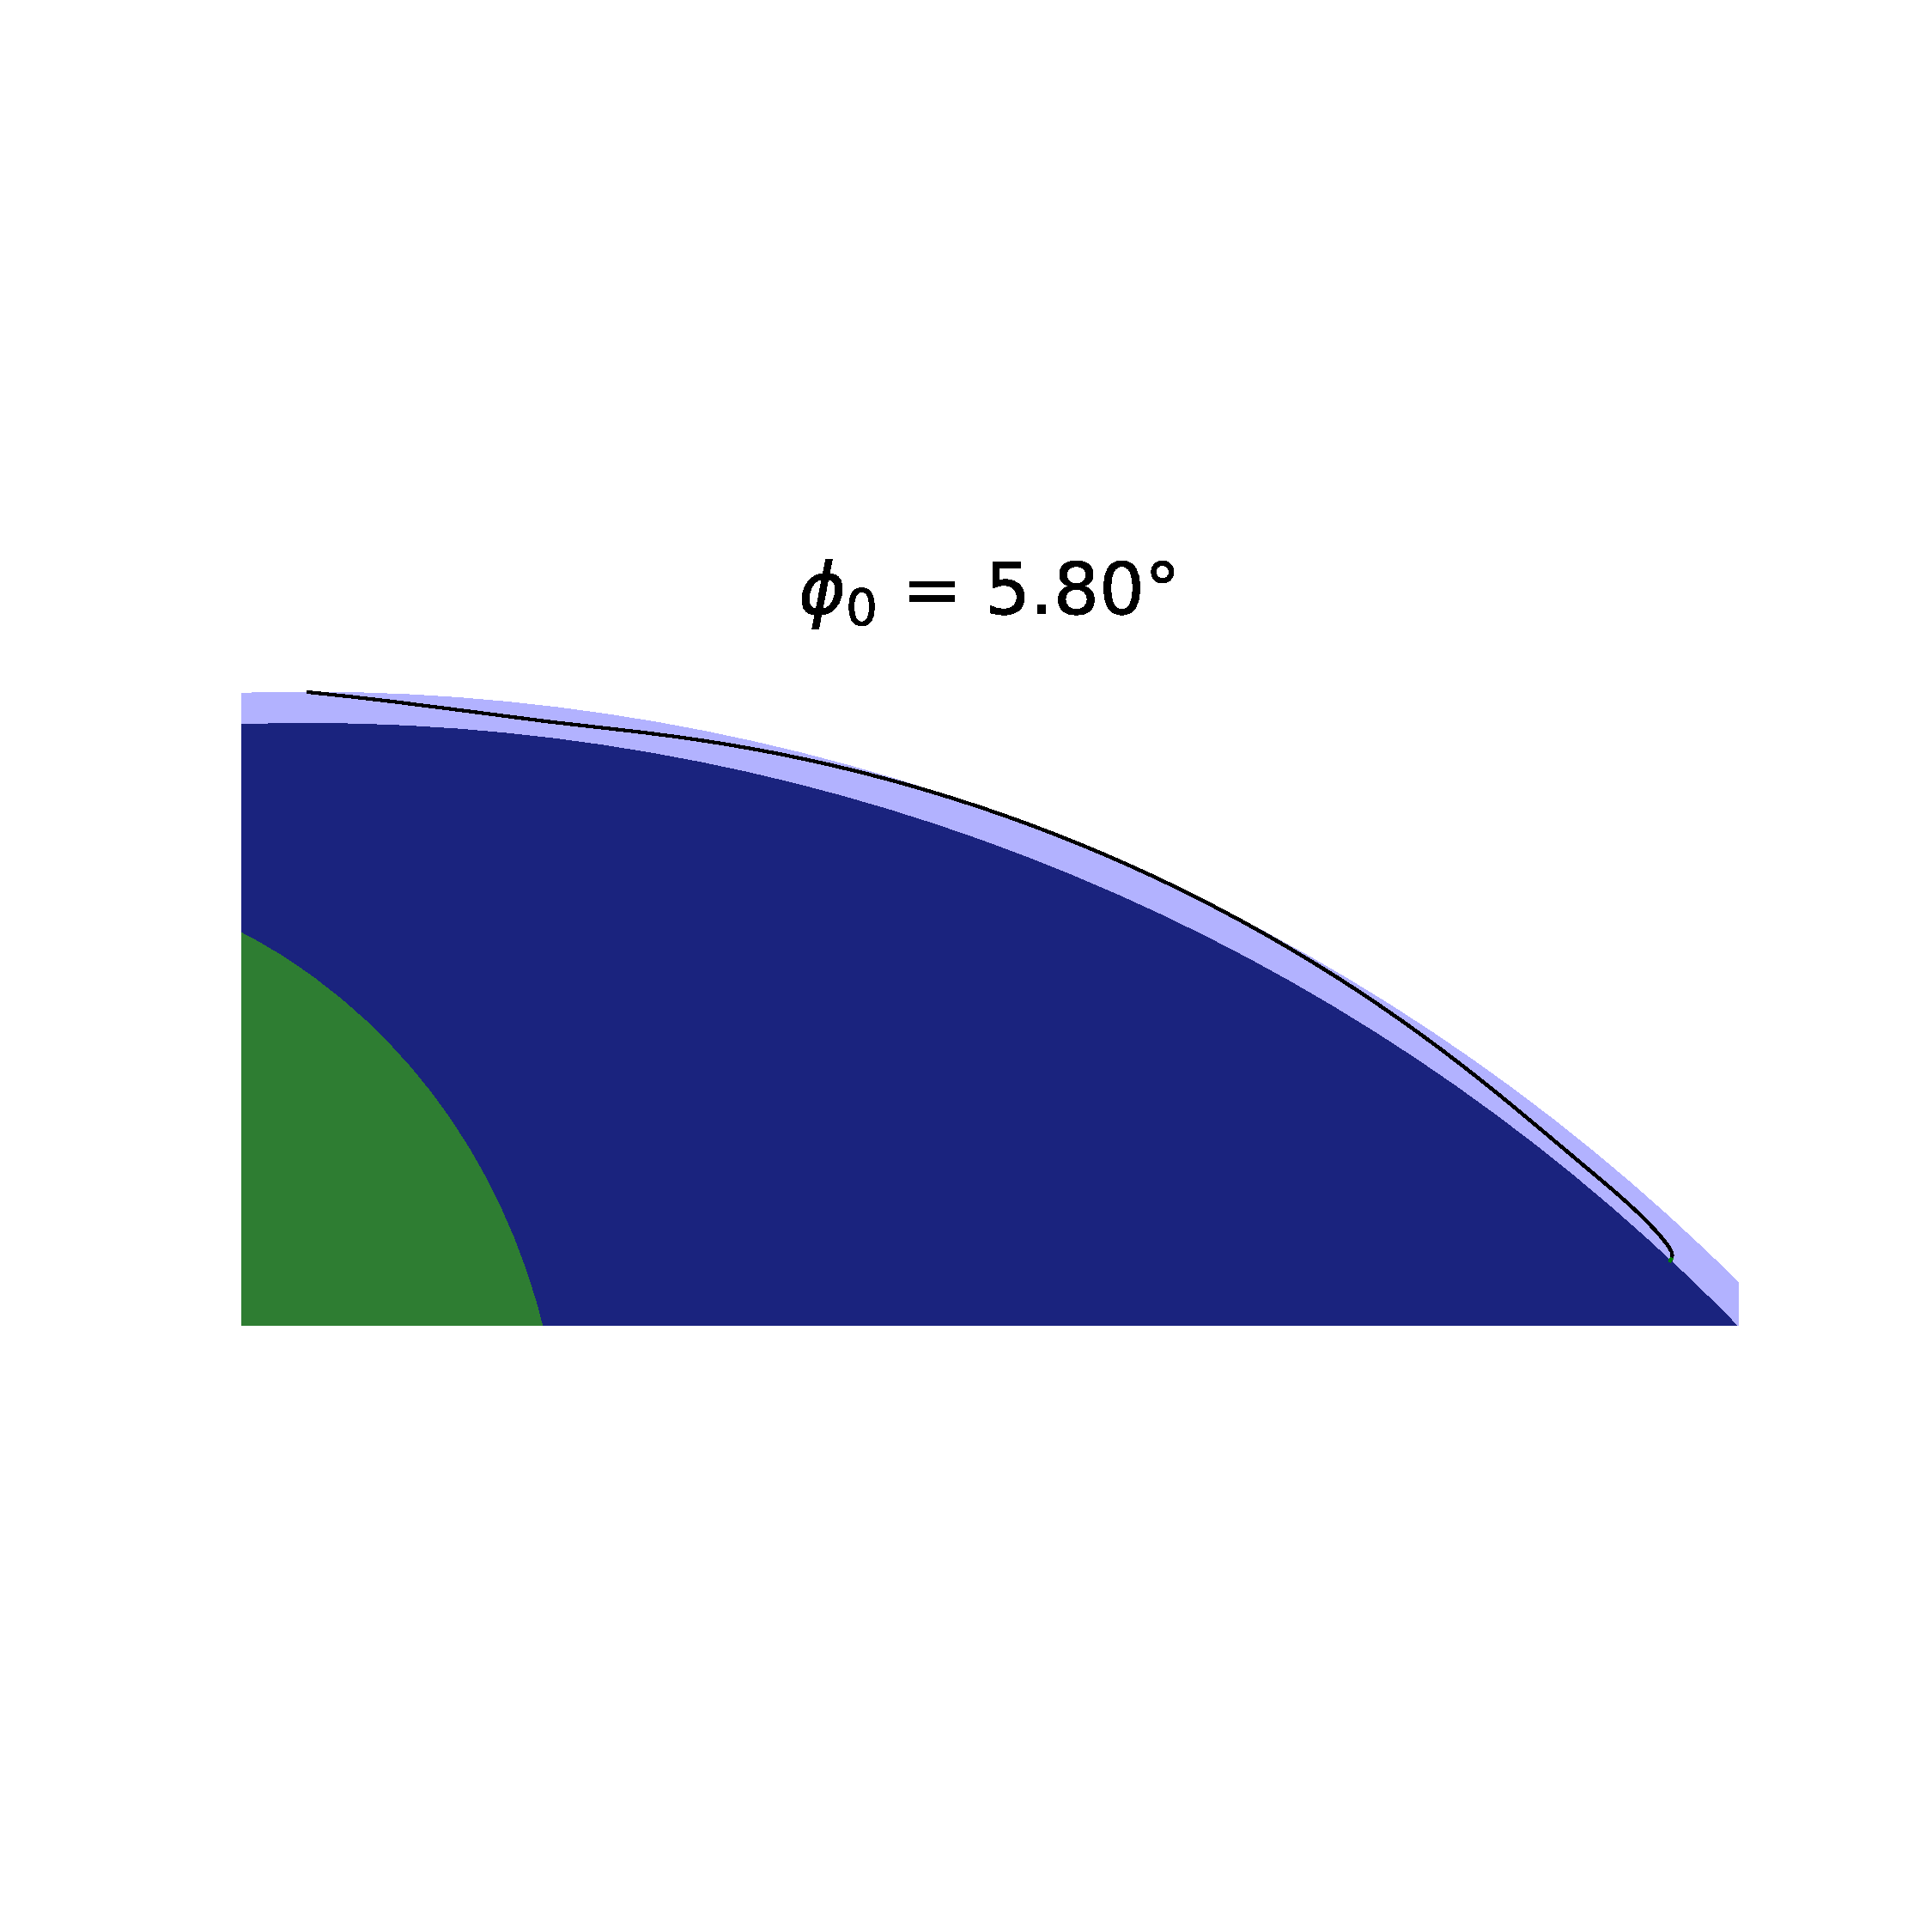
\includegraphics[width=12cm]{5_8_scheme.pdf}
		\caption{Skica povratka kapsule v atmosfero pri vstopnem kotu $ 5.8^\circ $}
	\end{center}
\end{figure}

Razliko med izra\v cunanim in pravim vstopnim kotom bi najverjetneje lahko pojasnili z nenatan\v cnostjo na\v sega modela. Model uporablja zelo grobo aproksimacijo za lastnosti atmosfere v odvisnosti od vi\v sine ter temperature. Veliko negotovost vna\v sata tudi koeficient sile upora in razmerje med silama vzgona ter upora. Ta dva se z temperaturo zraka, vi\v sino ter hitostjo gotovo spreminjata, model pa predpostavlja, da sta konstantna.

V simulaciji smo privzeli, da je kapsula samo objekt, ki pada nazaj v atmosfero. Pri resni\v cnem povratku pa kapsule niso brez vpljiva na svojo pot. Z majhnimi raketnimi motorji spreminjajo svoj naklon ter s tem vpljivajo na razmerje med silama vzgona in upora. Tako lahko popravijo manj\v se napake pri vstopnem kotu ter prakti\v cno neodvisno od vetra pristanejo v radiju nekaj kilometrov od \v zeljenega pristajali\v sca. To po\v cnejo vse dandanes lete\v ce kapsule, poseben primer tovrstnega manevriranja pa je raketoplan, ki spada \v ze v re\v zim letenja \cite{raketoplan-wiki}.

\subsection{Vstopni kot v odvisnosti od za\v cetne hitrosti}

Minimalen in maksimalen vstopni kot se glede na za\v cetno histrost mo\v cno spreminja. Iz grafa je razvidno, da se Apollo kapsule vra\v cajo v atmosfero pri hitrostih, kjer je interval \v sirok priblji\v zno $ 1^\circ $. \v Sirina intervala sprejemljivih vstopnih kotov se s pove\v cevanjem vstopne hitrosti drasti\v cno o\v za, pri histrostih ve\v cjih od $ 11800\ m/s $ pa kapsule ni mogo\v ce ve\v c pristati brez predhodnega zaustavljanja.

\begin{figure}[H]
	\begin{center}
		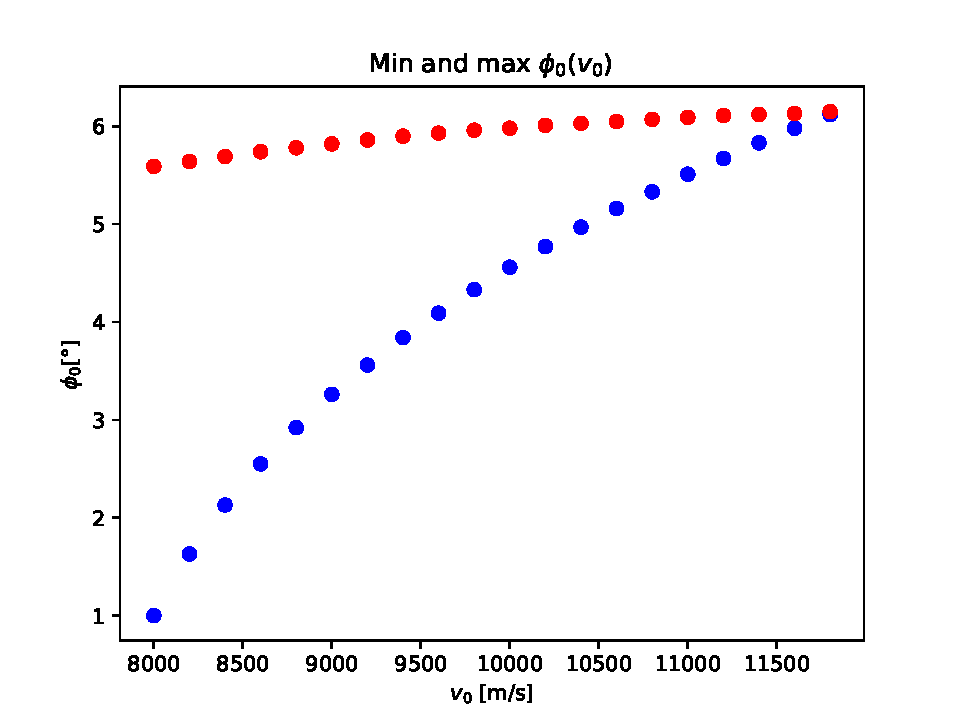
\includegraphics[width=12cm]{range_of_velocity.pdf}
		\caption{Minimalen in maksimalen vstopni kot v odvisnosti od za\v cetne hitrosti}
	\end{center}
\end{figure}
\clearpage

\subsection{Odboj od atmosfere}

Pri premajhnih vstopnih kotih se kapsula navadno od atmosfere odbije in poleti globoko v vesolje. V posebnih primerih se kapsula tudi po odboju vrne in s primernim kotom ponovno vstopi v atmosfero. Tak primer dveh odbojev je naprimer kot $ \phi_0 = 4.13^\circ $.

\begin{figure}[H]
	\begin{center}
		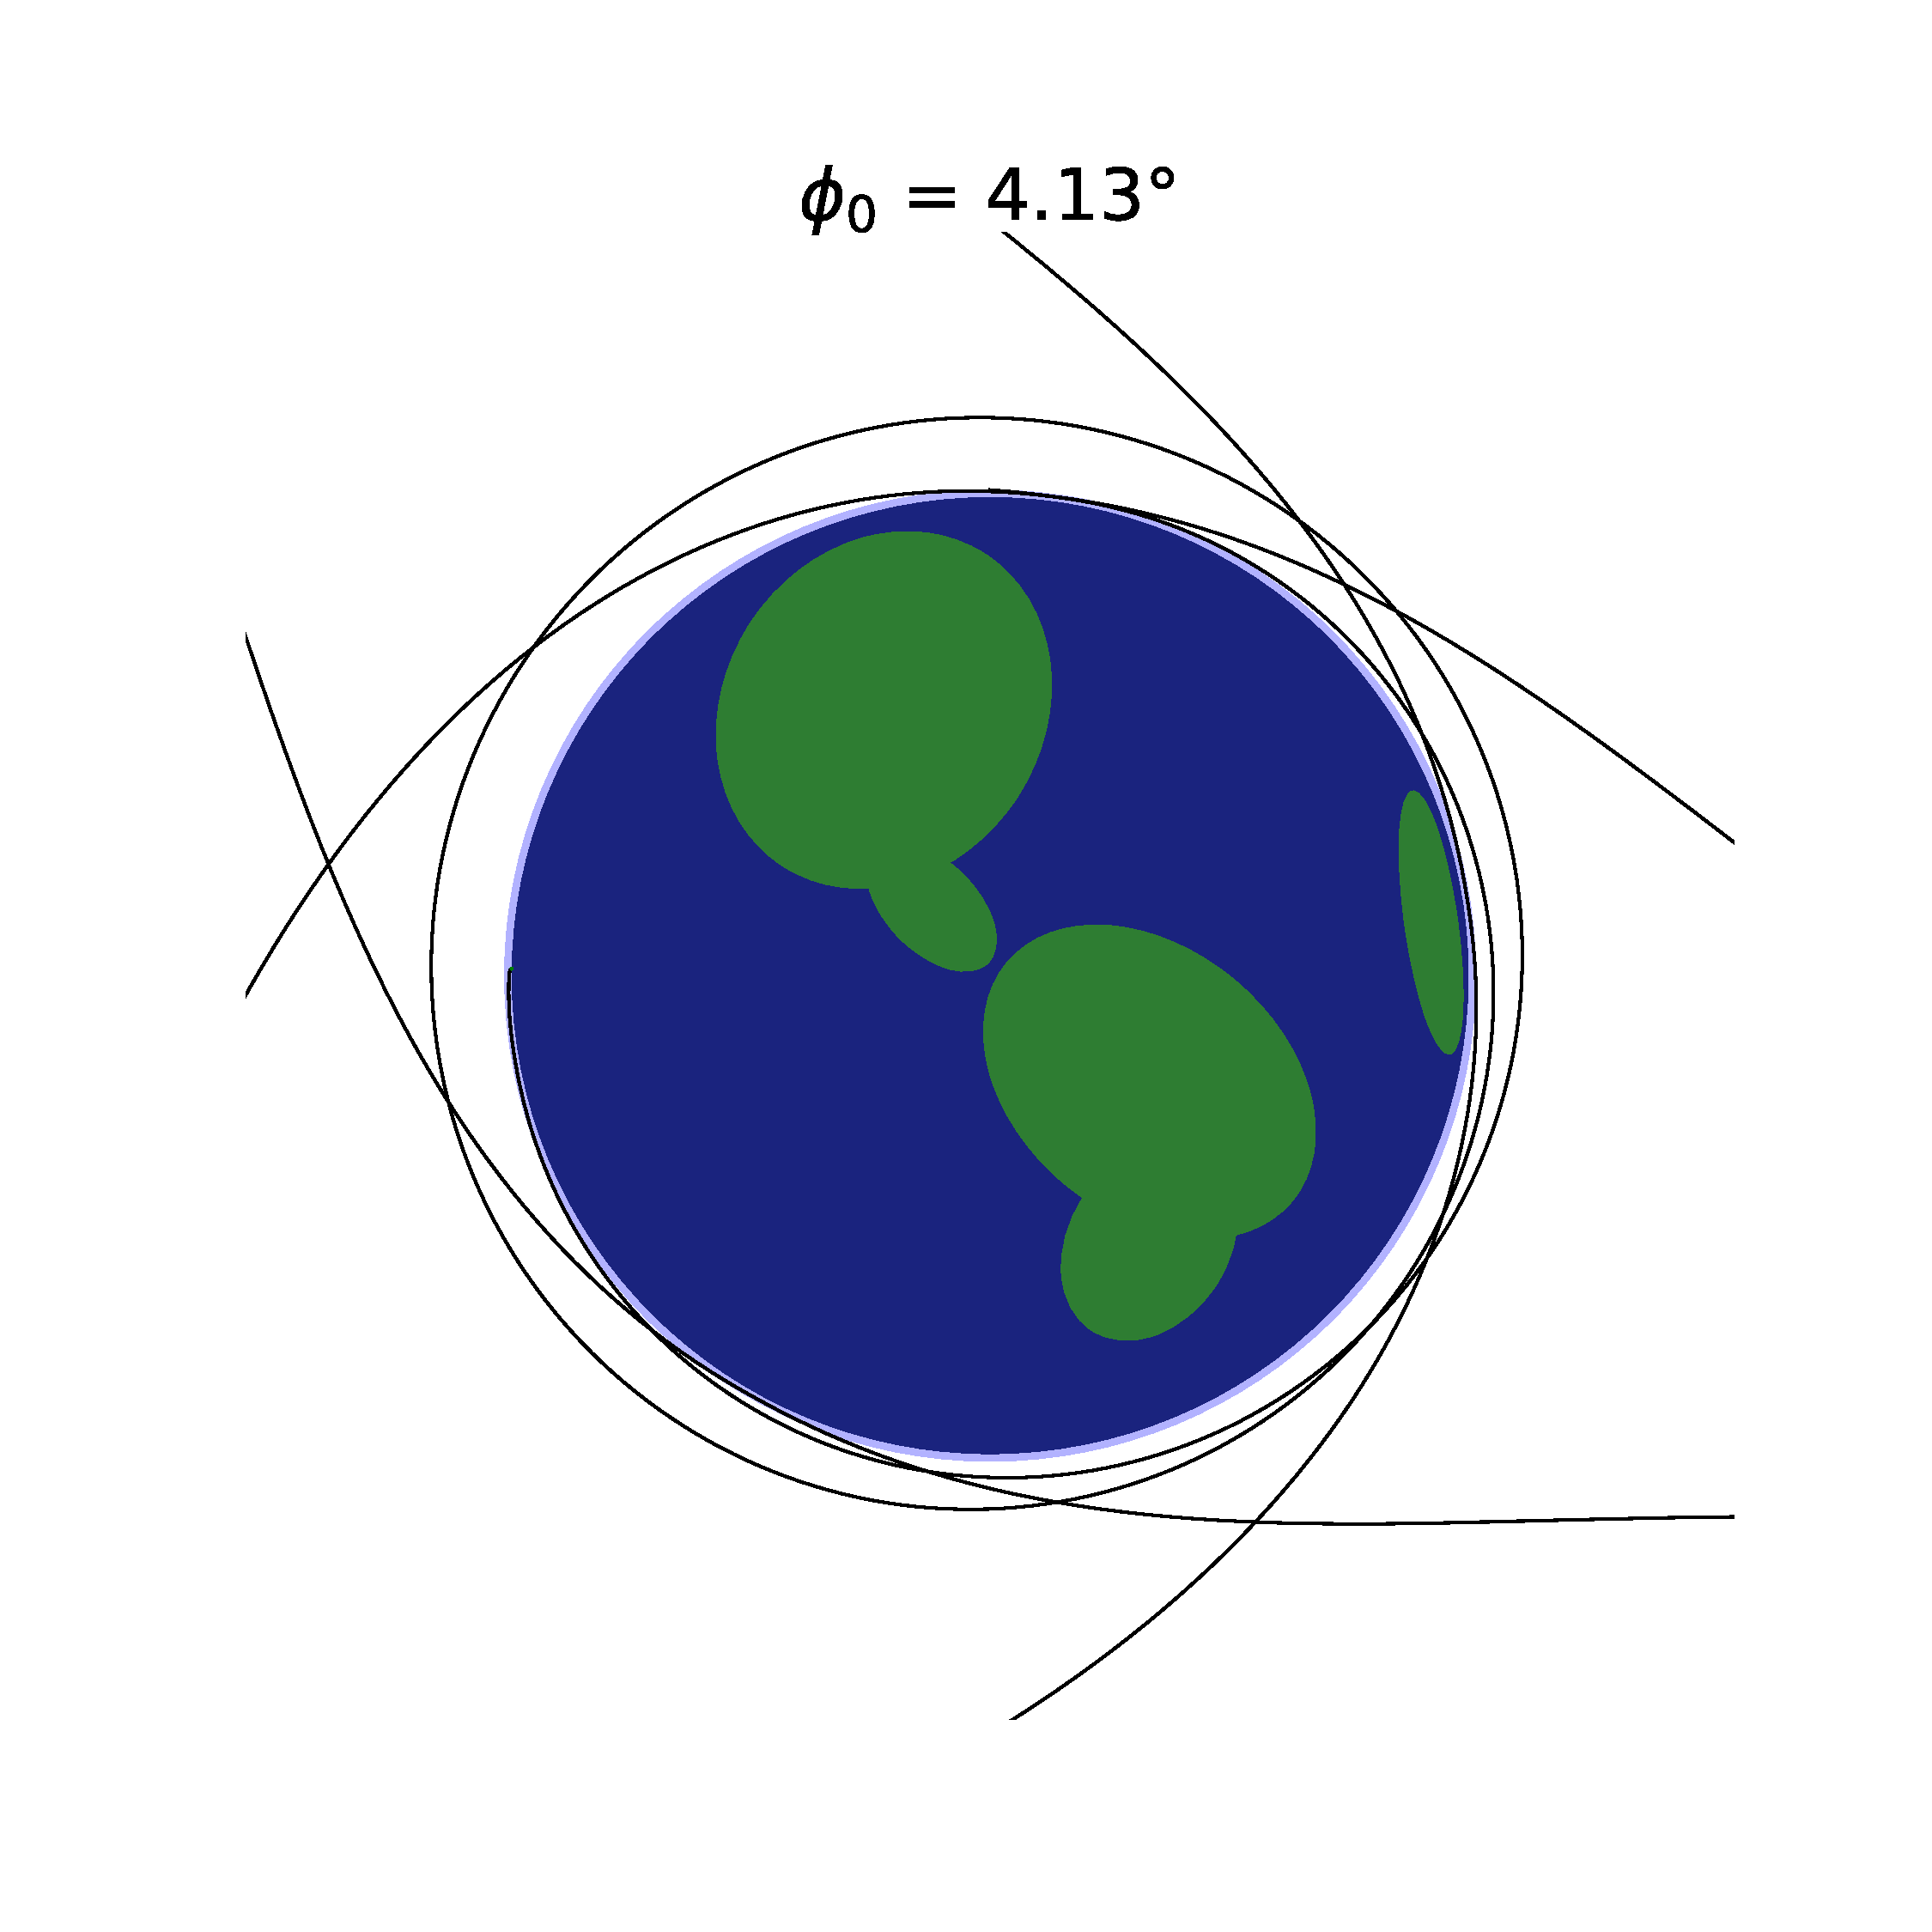
\includegraphics[width=12cm]{4_13_scheme.pdf}
		\caption{Primer dvojnega odvoja od atmosfere}
	\end{center}
\end{figure}

Tako odbijanje od atmosfere pa je, \v ceprav bi morda ustrezalo na\v sim kriterijem za maksimalno mo\v c in pospe\v sek, zelo nevarno. Astronavti so dlje \v casa v vesolju, potujejo po nekontrolirani in nena\v crtovani poti ter ne morejo vpljivati na kot ponovnega vstopa.
\clearpage

\section{Zaklju\v cek}
Varen povratek kapsule iz vesolja je eden najve\v cjih problemov poletov astronavtov v vesolje. Zaradi nere\v senega problema zaustavitve kapsule je Jurij Gagarin, prvi \v clovek v vesolju, iz kapsule moral sko\v citi s padalom z vi\v sine $ 7\ km $ \cite{vostok-1-wiki}. Ta problem so kasneje re\v sili, \v se dandanes pa povratek ostaja eden najnevarnej\v sih delov poletov v vesolje.

V tej projektni nalogi smo uspe\v sno zasnovali grobo simulacijo tovrstnega povratka ter izra\v cunali primerne vstopne kote. Te le rahlo odstopajo od pravih podatkov za kapsulo Apollo 4.

Simulacijo bi lahko nadgradili z natan\v cnej\v sim aerodinami\v cnim modelom kapsule in atmosfere. Velik dodatek bi bil zasnova sistema za vodenje kapsule pri ponovnem vstopu in \v cimnatan\v cnejsem pristajanju. Simulacijo pa za zabavo lahko uporabimo tudi na drugih planetih.

%\vspace{1cm}

%\begin{figure}
%  \begin{center}
%  	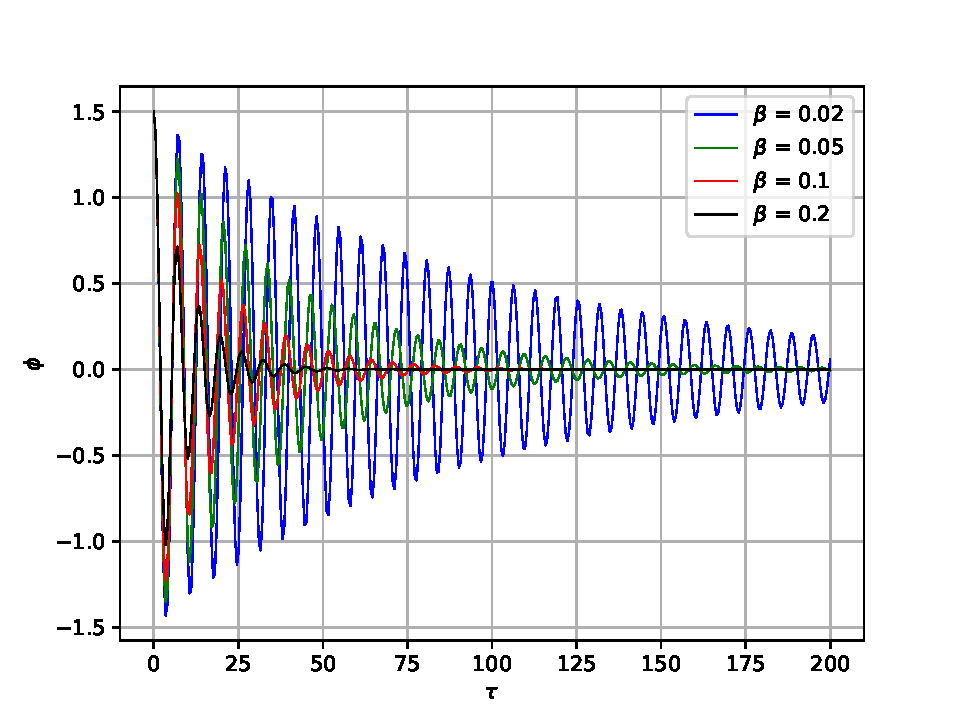
\includegraphics[width=12cm]{graf1.pdf}
%    \caption{Graf $\phi$ v odvisnosti od $\tau$}
%  \end{center}
%\end{figure}
%
%\begin{figure}
%  \begin{center}
%  	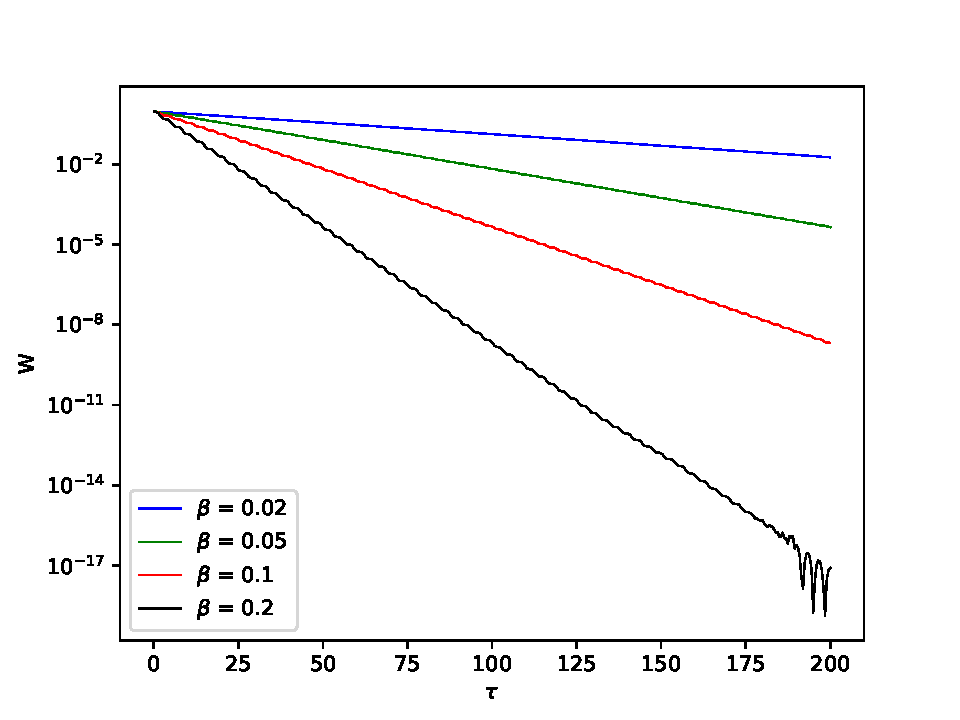
\includegraphics[width=12cm]{graf2.pdf}
%    \caption{Graf energije v odvisnosti od $\tau$ v logaritmski skali}
%  \end{center}
%\end{figure}

\vspace{2cm}


\clearpage
\section{Literatura}
\printbibliography[heading=none]
\end{document}
